\documentclass{article}
\date{February 2019}
\author{Joe Singleton}
\title{
    Notes on theory of truth discovery
}

% Packages:
\usepackage{amsmath}
\usepackage{amsthm}
\usepackage{caption}
\usepackage{cite}
% \usepackage[top=2cm, bottom=2cm, left=3cm, right=3cm]{geometry}
\usepackage{graphicx}
\usepackage{hyperref}
\usepackage{multicol}
\usepackage{charter}  % For cool font
\usepackage{xcolor}

\graphicspath{ {./images/} }

% Settings
\hypersetup{
	colorlinks,
	citecolor={blue!80!black},
	urlcolor={blue!80!black},
	linkcolor={blue!80!black}
}

% Maths environments
\theoremstyle{definition} \newtheorem{definition}{Definition}
\theoremstyle{definition} \newtheorem{example}{Example}
\theoremstyle{plain} \newtheorem{axiom}{Axiom}
\theoremstyle{plain} \newtheorem*{remark}{Remark}
\theoremstyle{remark} \newtheorem*{notation}{Notation}
\theoremstyle{plain} \newtheorem{lemma}{Lemma}
\theoremstyle{plain} \newtheorem{proposition}{Proposition}

% Commands
\newcommand{\todo}[1] {
    \textcolor{red}{
        \textbf{TODO:} #1
    }
}
% Sets
\renewcommand{\S}{\mathcal{S}}  % Note: overrides existing command
\renewcommand{\O}{\mathcal{O}}  % Note: overrides existing command
\newcommand{\F}{\mathcal{F}}
\newcommand{\N}{\mathcal{N}}
% Source and fact orderings: less-equal, less-than, greater-equal, equal
\newcommand{\sle}{\sqsubseteq}
\newcommand{\slt}{<}
\newcommand{\sge}{\ge}
\newcommand{\seq}{\simeq}
\newcommand{\fle}{\preceq}
\newcommand{\flt}{\prec}
\newcommand{\fge}{\succeq}
\newcommand{\feq}{\approx}

\newcommand{\src}{\texttt{src}}
\newcommand{\fact}{\texttt{facts}}
\newcommand{\obj}{\texttt{obj}}
\newcommand{\orderings}{\mathcal{L}}

\begin{document}
\maketitle
% \begin{multicols}{2}

\section{Frameworks for truth-discovery used in existing literature}
\label{sec:existing_frameworks}

\subsection{Li et. al. survey}
\label{sec:li}

A 2015 survey by Li et. al. {\cite{li_survey}} defines truth-discovery as
follows.

\begin{itemize}
\item We have a set of sources $\S$, and a set of objects $\O$
\item Each source $s$ claims a value $v_{o}^{s}$ for some objects $o$ (not
necessarily \emph{all} objects)
\item Truth-discovery: compute a \emph{source weight} $w_s$ for each source,
and compute `truth values' $v_{o}^{*}$ for each object $o$
\item \emph{Single truth assumption}: there is exactly one true value for each
object. This may not always hold (e.g. consider which actors star in a film)
\end{itemize}

\subsection{Gupta and Han survey}
\label{sec:gupta}

From \cite{gupta_han_survey}, slightly re-phrased by me (e.g. paper calls
sources `providers', denotes confidence by $s$\ldots)

\begin{itemize}
\item Set of sources $\S$, objects $\O$
\item Each object $o$ has as associated set of \emph{facts} $F_o$. Write
$\F = \bigcup_{o \in \O}F_o$
\item Sources \emph{provide} facts about objects. They may provide facts about
multiple objects, but only one fact per object
\item Could be formalised similar to \ref{sec:li} as follows: $f_o^s \in F_o$
is the fact provided by source $s$ for object $o$, defined for a subset of $\O$
\item Truth-discovery: compute \emph{source trusts} $t_s$ for each source $s$,
and \emph{fact confidence} $c_f$ for each fact $f$
\end{itemize}

Note that general set up is more or less equivalent to in \ref{sec:li}: facts
replace values. However the definition of a truth-discovery algorithm is
different: here each fact is given a confidence score, whereas in \ref{sec:li}
we only find the most believable fact for each object.

If each fact is given a confidence score then it is simple to find most
believed fact for each object by taking the fact with highest confidence.

\subsection{Latent Dirichlet Truth Discovery}
\label{sec:ldt}

The method proposed in \cite{zhang_qi_tang} is similar to both above approaches:

\begin{itemize}
\item Set of sources $\S$, objects $\O$, facts $F_o$ for each $o \in \O$
\item Each source $s$ makes claim $\texttt{Cl}_o(s) \in F_o \cup
\{\oslash\}$ for the true fact for object $o$, where $\oslash$ is special
symbol to indicate no claim is made
\item Each source has a \emph{trustworthy component} and \emph{untrustworthy
component}
\item Truth-discovery:
    \begin{itemize}
    \item Compute probability that each fact $f$ is the true fact for its
    associated object (i.e. confidence in each fact?)
    \item Compute trustworthy and untrustworthy amounts in each source
    (trustworthy amount can be considered source trustworthiness, comparable to
    other approaches)
    \end{itemize}
\end{itemize}

\subsection{Pasternack and Roth}
\label{sec:past}

In \cite{pasternack}:

\begin{itemize}
\item Set of sources $\S$, each with a set of claims $C_s$ ($s \in \S$). Write
$\mathcal{C} = \bigcup_{s \in \S}{C_s}$
\item Each claim $c$ has \emph{mutual exclusion} set $M_c \subseteq
\mathcal{C}$: only one claim in each $M_c$ is true. Note that $c \in M_c$
\item Truth-discovery: compute source trusts $t_s$ and claim beliefs $b_c$
\end{itemize}

This is essentially the same as \ref{sec:gupta}, if we let each mutual
exclusion set be called an object, rename claims to facts, and the facts
provided by source $s$ are simply those in $C_s$. Something like the following.
$$
\O = \{M_c : c \in \mathcal{C}\},
\quad
F_{M_c} = M_c
$$

The only slight problem is that under this mapping a fact (\ref{sec:gupta}
sense) may be related to multiple objects, e.g. if $c \in M_{c'}$ but $M_c \ne
M_{c'}$.

\subsection{Galland et. al algorithms}
\label{sec:galland}

Several algorithms are proposed in \cite{galland}, and each uses the following
scheme, which is initially quite different from those above (again, slightly
re-phrased by me in places):

\begin{itemize}
\item Set of sources $\S$, facts $\F$, and the \emph{real world}
$W: \F \rightarrow \{\texttt{True}, \texttt{False}\}$
\item Each source $s$ is a partial mapping $\F \rightarrow
\{\texttt{True}, \texttt{False}\}$
\item Each source $s$ has an \emph{error factor} $\epsilon(s) \in [0, 1]$ (?)
that represents the likeliness of $s$ making a mistake on the truth value of
any given fact
\item Set of \emph{queries} $\mathcal{Q}$. Each fact $f$ has a \emph{reference
query} $ref(f) \in \mathcal{Q}$ (imagine that $q\in\mathcal{Q}$ is a question,
and $f$ answers the question in some way). Any query has exactly one true fact.
Formally, for each query $q$, let $F_q = \{f \in \F : ref(f) = q\}$.
For each $q$ there is exactly one $f \in F_q$ with $W(f) = \texttt{True}$ \item
Truth-discovery: compute source error factors $\epsilon(s)$, and an estimate
for the real world $W$ given as a mapping $\F \rightarrow [0, 1]$ where 1
represents true and 0 represents false.
\end{itemize}

Some important differences here:
\begin{itemize}
\item Sources may claim a fact is \emph{false}, which is not possible in the
other approaches
\item Objects are not first-class citizens
\item Notion of queries. The set of queries (along with the reference query for
each fact) is not given as input to algorithms; it is instead used to produce a
modified set of views, where for each source $s$ and each fact $f$ such that
$s(f) = \texttt{True}$, we add a new claim $s(f')=\texttt{False}$ for each
$f' \ne f$ such that $f'$ and $f$ relate to the same query. This idea is
applicable whenever the \emph{single truth assumption} is assumed, but only for
algorithms that consider negative facts. See section 3 of \cite{galland} for
details.
\end{itemize}

I think we can view this model as a special case of the one in \ref{sec:li},
where objects (\ref{sec:li} sense) are facts, and $v_f^s$ (\ref{sec:li} sense)
is given by $s(f)$ (\ref{sec:galland} sense, when this is defined).

This is a special case since the only claimed values are \texttt{True} and
\texttt{False}, whereas in \ref{sec:li} the values can be anything.

\section{Extensions to basic truth-discovery}
\begin{itemize}

\item Implications between facts about the same object{\cite{yin_han_yu}}
\item Incorporating prior knowledge{\cite{pasternack}}
\item Considering difficulty of facts{\cite{galland}}
\item Heterogeneous data (i.e. possible values for an object are not all
categorical, and can be different types){\cite{li_conflicts}}
\item Correlations between objects{\cite{yang}}
\item Considering that for some questions there is no true answer (objects have
no true facts){\cite{zhi}}
\item Supervised truth-discovery (some ground truths are
known){\cite{yin_supervised}}
\item Truth changing over time, and sources copying from other
sources{\cite{dong}}
\item Truth-discovery in data streams, where source claims arrive continuously
over time{\cite{zhao}}

\end{itemize}

\section{Ideas for axioms}

\subsection{Existing work}

\begin{itemize}

\item \emph{Trust-based recommendation systems: an axiomatic
approach}{\cite{andersen}}. In a trust-based recommendation system
\emph{agents} trust other agents, and a subset of the agents (the
\emph{voters}) have expressed an opinion about some item of interest: votes are
either $+$ or $-$. The goal is to assign recommendations $+$, $-$ or $0$ to the
\emph{non-voters} using the trust relationships between agents.

The network here is \emph{homogeneous} as all nodes in the graph are agents,
and agents trust each other. This is in contrast with truth-discovery where
edges are between entities of different types.

The recommendations are also \emph{personalised} which is not applicable to
truth-discovery, since we want to find the global truths.

Nevertheless the paper gives some axioms that seem like they could be
applicable.

\item Judgement aggregation (handbook 17.2) seems highly relevant.

\item \emph{An Axiomatic Approach to Personalised Ranking
Systems}{\cite{altman_personalised}}. Agents trust other agents, represented as
directed edges in a graph. A personalised ranking system gives a ranking of the
agents \emph{for each agent}. Each ranking depends on which agents are trusted.

Has interesting transitivity-type axioms that sound highly applicable to
truth-discovery: if a fact $f_1$ has sources that are `more trusted' than the
sources of $f_2$ (where $f_1, f_2$ relate to the same object), then $f_1$
should be more believed than $f_2$.

E.g. similar to `quasi-transitivity' in the paper: if there is a bijection $p$
between sources for $f_1$ and $f_2$ such that $s$ is more trusted than $p(s)$
for all sources $s$ of $f_1$, then $f_1$ is believed more than $f_2$.

The paper allows this for $p$ injective but not necessarily surjective. I don't
think would work for truth-discovery sine the addition of a very bad source
could (righly) bring a fact's belief down, even if its other sources were
better.

There can be a dual property where sources and facts are swapped.

\item \emph{Group Recommendations: Axioms, Impossibilities, and Random
Walks}{\cite{lev}}. Set up is similar to trust-based, but recommendations are
given to \emph{sets} of agents.

\item General social choice (e.g. see Handbook chapter 1 for overview). It
sounds like the fact ordering part of truth-discovery could be a special case
of a social welfare function, where sources rank their claims strictly above
all others (but they would have to rank their own facts equally\ldots).

\end{itemize}

It seems like there is a lot of existing work on things like ranking systems,
aggregating preferences of a group (social choice) which have similarities with
truth-discovery.

\subsection{Ideas for truth-discovery}
\begin{itemize}

\item Independence of irrelevant claims: if a subset of sources, objects, facts
is not connected to the rest of the graph, then changes outside this subset
should not affect the results on the subset.

\item Consensus-type axiom: if all sources claim $f$, then $f \fge f'$ for all
$f' \ne f$. Or on a per-object basis: if $o = O_f$ and $(s, f) \in E$ for all
$s \in \S_o$ then $f \fge f'$ for $f' \in F_o \setminus \{f\}$.

Both only make sense if we allow facts that are not claimed by anyone. Compare
to \emph{weakly Paretian} in Handbook to COMSOC, p6.

\item As sort of a dual notion to the above: if a fact is ranked highest (for
an object, or overall) then it must have been claimed by at least one source.
This is similar to an axiom in judgement aggregation. \todo{find the JA
version}

\item Principle that trustworthy sources claim believable facts, and vice
versa: see `quasi-transitivity' above and in \cite{altman_personalised}.

Roughly, this would involve taking two facts, and comparing their sources in
some way. If one set of sources is `more trustworthy', the corresponding fact
should be more believable than the other. This could be for two facts about the
same object, or any two facts.

The other direction would be similar.

This would imply that sources with the same facts (respectively, facts with the
same sources) are ranked equally. This equality version could perhaps be
stated as a weaker version of the above.

\item Making many false claims should not improve trust ranking (this is the
problem that \emph{Average${\cdot}$Log} tackles)

\item If a source claims a new fact better than all its current ones, its trust
ranking should not get worse. Also, if the new fact is worse, its trust ranking
should not go up.

Dual axiom for facts: if a new source is added that ranks higher for trust than
existing sources for a fact, that fact's belief ranking should not get worse.
Similar for opposite situation.

\textbf{Note:} Under definition \ref{def:truth_discovery_operator} only the
\emph{relative} position of sources can be judged as getting better or worse.
Something like the following would check if $s$ gets worse than \emph{some}
other source after a change: $s$ ranks worse in $N'$ than in $N$ if there is
$s' \in \S$ such that $s' <_N s$ and $s \sle_{N'} s'$.

Or we could assign each source a number according to which position they rank,
and use this number to compare positions after a change in input.

\item Consider changing a network's graph from $G$ to $G'$ and $G''$ where in
$G'$ we add to a source $s$ a fact $f'$, and in $G''$ we add $f''$. If $f'
\fle_G f''$ then $s$'s ranking should not be better in $G'$ than in $G''$.

This seems similar to the previous idea. It has the same problem with
\emph{how} we measure when a source is worse when comparing on different graphs.

\end{itemize}

\section{Theory of truth-discovery}

The input seems to be essentially equivalent in all approaches listed in
section \ref{sec:existing_frameworks}, with the exception of \ref{sec:galland}
which has the concept of negative claims.

Output differs: in \ref{sec:li} a single true fact is selected for each object,
and in the others all facts are given a belief score in $[0, 1]$. Both
approaches ultimately \emph{rank} the facts of each object.

The framework I choose should be general enough that all (or at least most)
algorithms in the literature can fit into it. The framework will then
facilitate comparison between the algorithms.

First we state some standard definitions, and then give a graph-theoretic
formulation of truth-discovery.

\subsection{Standard definitions}

\begin{definition}
A \emph{relation} $R$ on a set $X$ is a subset $R \subseteq X \times X$. We
use the infix notation $x \mathbin{R} y$ to mean $(x, y) \in R$.
\end{definition}

\begin{definition}
A \emph{preorder} on a set $X$ is a relation $\preceq$ that is reflexive and
transitive:
\begin{enumerate}
\item $x \preceq x$ for all $x \in X$ (reflexivity)
\item If $x \preceq y$ and $y \preceq z$, then $x \preceq z$ for all $x, y, z
\in X$ (transitivity)
\end{enumerate}

A \emph{total preorder} is a preorder that is complete: for all $x, y \in X$,
$x \preceq y$ or $y \preceq x$. $\orderings(X)$ is the set of all total
preorders on $X$.

The \emph{strict} order induced by $\preceq$ is $\prec$ where $x \prec y$ if
and only if $x \preceq y$ but not $y \preceq x$. Note that $\prec$ is
irreflexive, transitive (and hence asymmetric), and is not complete.

The \emph{equality predicate} associated with $\preceq$ is $\simeq$, where $x
\simeq y$ if and only if $x \preceq y$ and $y \preceq x$. Note that $\simeq$ is
an equivalence relation on $X$.

\end{definition}

\begin{definition}
A \emph{permutation} of a set $X$ is a bijective mapping $X \rightarrow X$. We
use cyclic notation for permutations: $\pi=(a, b, c)$ is the mapping $\pi(a) =
b$, $\pi(b) = c$, $\pi(c) = a$, and $\pi(x) = x$ for $x \notin \{a, b, c\}$.
Juxtaposition of cycles denotes function composition. It is well known that any
permutation can be expressed as a composition of disjoint cycles.\todo{find
source for this if it will actually be used anywhere.}
\end{definition}

\begin{definition}
For any set $X$, relation $R \subseteq X \times X$, and permutation $\pi: X
\rightarrow X$, we denote by $\pi(R)$ the relation
$$ \pi(R) = \{(\pi(x), \pi(y)) : x \mathbin{R} y\} $$
That is, $(u, v) \in \pi(R)$ if and only if $(\pi^{-1}(u), \pi^{-1}(v)) \in R$.
\end{definition}

Note that if $R$ is an total preorder then so too is $\pi(R)$. If we view $\pi$
as relabelling the elements of $X$, then $\pi(R)$ is the same ordering as $R$,
but given in terms of the new labels.

\begin{definition}

Two graphs $G=(V, E)$ and $G'=(V', E')$ are \emph{isomorphic} if there is a
bijective mapping $\phi: V \rightarrow V'$ such that $(u, v) \in E \iff
(\phi(u), \phi(v)) \in E'$.

\end{definition}

\begin{definition}
Let $G=(V, E)$ be an undirected graph, and define a relation $\sim$ on $V$ by
$u \sim v$ iff there is a path from $u$ to $v$ in $G$ (including the
zero-length path when $u = v$). It is easily checked that $\sim$ is an
equivalence relation. A \emph{connected component} of $G$ is an induced
subgraph of an equivalence class of $\sim$.
\end{definition}

\subsection{Truth-discovery definitions}

We consider fixed finite sets $\S$, $\F$ and $\O$, called the \emph{sources},
\emph{facts} and \emph{objects} respectively. All definitions and axioms will
be stated with respect to these sets.

% Input network definition
\begin{definition}

A \emph{truth-discovery network} is a directed graph $N = (V, E)$ where $V = \S
\cup \F \cup \O$, and $E \subseteq (\S \times \F) \cup (\F \times \O)$
satisfies the following properties:

\begin{enumerate}
\item Each $f \in \F$ has a unique successor node in $\O$, denoted $\obj(N, f)$
(i.e. each fact relates to a single object).

\item For $s \in \S$ and $o \in \O$, there is at most one directed path from
$s$ to $o$ (i.e. sources can only claim one fact per object).

\item $(\S \times \F) \cap E$ is non-empty (i.e. at least one claim is made).

\end{enumerate}
We will say that $s$ \emph{claims} a fact $f$ when $(s, f) \in E$. Let $\N$
denote the set of all truth-discovery networks.
\end{definition}

\begin{remark}
Note that the definition above does not rule out a source $s$ making no claims,
a fact $f$ being claimed by no sources, or an object $o$ having no associated
facts or sources.

In the special case where each object has exactly two associated facts, the
objects can be seen as \emph{binary variables} taking one of two values, e.g.
true or false. The truth-discovery network is then similar to a set of
judgements in \emph{judgement aggregation}\cite{handbook_ja} for an agenda
consisting only of propositional variables.
\end{remark}

\begin{notation}
For convenience, for a network $N=(V, E)$, define:
\begin{align*}
    \fact(N, s) &= \{f \in \F : (s, f) \in E\} \\
    \fact(N, o) &= \{f \in \F : (f, o) \in E\} \\
    \src(N, f) &= \{s \in \S : (s, f) \in E\} \\
    \src(N, o) &= \{s \in \S : \exists f \in \F : (s, f), (f, o) \in E\} \\
\end{align*}
\end{notation}

% Algorithm definition
\begin{definition}
\label{def:truth_discovery_operator}

A \emph{truth-discovery operator} $T$ is a mapping $T: \N \rightarrow
\orderings(\S) \times \orderings(\F)$, i.e. $T$ assigns to each truth-discovery
network a pair of total preorders $T(N) = (\sle_N^T, \fle_N^T)$ on the sets
$\S$ and $\F$ respectively.

$s_1 \sle_N^T s_2$ means $s_2$ is ranked as \emph{more trustworthy} than $s_1$
in the network $N$ according to $T$; $f_1 \fle_N^T f_2$ means $f_2$ is ranked
as \emph{more believable} than $f_1$. Sub- and super-scripts can be omitted
when clear from context.

\end{definition}

\begin{definition}
\label{def:numerical}

A \emph{numerical truth-discovery operator} $T$ assigns to each
truth-discovery network $N$ a \emph{source trust} mapping $\tau: \S \rightarrow
[0, 1]$ and \emph{fact belief} mapping $\phi: \F \rightarrow [0, 1]$.

\end{definition}

\begin{remark}
    Any numerical truth-discovery operator $T$ naturally induces a
    truth-discovery operator $T'$, where for any truth-discovery network $N$
    we define
    \begin{align*}
    s_1 \sle_N^{T'} s_2 & \iff \tau(s_1) \le \tau(s2) \\
    f_1 \fle_N^{T'} f_2 & \iff \phi(f_1) \le \phi(f_2)
    \end{align*}
    for $s_1, s_2 \in \S$ and $f_1, f_2 \in \F$.
\end{remark}

In this work we deal primarily with truth-discovery operators as defined in
definition \ref{def:truth_discovery_operator}, instead of working directly
with numeric trust and belief scores. This is because we are interested in the
qualitative ranking of sources and facts, rather than quantitative values. This
approach is common in axiomatic treatment of ranking
systems{\cite{altman,altman_personalised}}. \todo{find more references for this
(e.g. Arrow, 1951, p17)}

Dispensing with numeric values is further justified by the fact that
trust/belief scores produced by numeric operators often do not have any
semantic meaning\cite{pasternack}, and so only the \emph{ranking} of
sources/facts is important.

One downside to this approach is that whilst we can tell whether or not $s_1$
is more trustworthy than $s_2$, we cannot tell by \emph{how much}.  For
example, consider two numeric operators $T$ and $T'$ and $\S=\{s_1, s_2\}$
such that $\tau(s_1)=0.5, \tau(s_2)=0.51$, and $\tau'(s_1)=0.01,
\tau'(s_2)=0.99$. Both operators induce the same ranking on $\S$, yet $T$
considers the two sources to have similar trust values while $T'$ considers
$s_2$ to be much more trustworthy than $s_1$.

\textbf{Notes:}
\begin{itemize}

\item Some operators only give most believed values as output (neither a
ranking nor belief score for each fact) (e.g. \cite{li_conflicts}). However we
can view such an operator in the above framework by considering it to rank the
discovered true facts above all others, and ranking false facts equally.

\item Some operators may give most-believed values for facts that are not
claimed by any sources, e.g. if values are continuous could perform a weighted
average of claimed facts (I believe this is done in \cite{li_conflicts} for
continuous data types). Neither of the definitions above support this.

\end{itemize}

\subsection{Axioms}

\subsubsection{Inspired by social choice}

The fact-believability component of truth-discovery can be seen as a special
case of voting in the theory of social choice, where agents are sources and
alternatives are facts. Each source then ranks the facts it claims above all
other facts, and ranks its claimed facts equally.\footnotemark

\footnotetext{
    Note that the formulation of social choice must allow for agents to have
    \emph{weak} preferences for alternatives, where ties are allowed.
}

Several axioms applicable to social welfare and social choice functions from
classical social choice can be directly adapted to truth-discovery.

\begin{definition}
Two truth-discovery networks $N$ and $N'$ are \emph{equivalent} if there is a
graph isomorphism $\pi$ between them that preserves sources, facts and objects:
\begin{enumerate}
\item $\pi(s) \in \S$ for all $s \in \S$
\item $\pi(f) \in \F$ for all $f \in \F$
\item $\pi(o) \in \O$ for all $o \in O$
\end{enumerate}

In such case we write $\pi(N)$ for $N'$.
\end{definition}

Figure \ref{img:permutation_of_a_tdn} shows an example of a permutation of a
truth-discovery network.

The first axiom states that the ordering of sources and facts should not depend
on the `names' of the sources, facts and objects in the input.

\begin{definition}
Let $T$ be a truth-discovery operator. $T$ satisfies \emph{symmetry} if for
any equivalent truth-discovery networks $N$ and $N' = \pi(N)$, we have
$$ s_1 \sle_N^T s_2 \iff \pi(s_1) \sle_{N'}^T \pi(s_2) $$
and
$$ f_1 \fle_N^T f_2 \iff \pi(f_1) \fle_{N'}^T \pi(f_2) $$

$T$ satisfies \emph{source-symmetry} if both the above statements hold in cases
where $\pi$ only permutes sources, i.e. $\pi(f)=f$ and $\pi(o)=o$ for all $f
\in \F$ and $o \in \O$. \emph{Fact-symmetry} and \emph{object-symmetry} are
defined similarly.
\end{definition}

\begin{axiom}(Symmetry)
An operator $T$ should satisfy symmetry.
\end{axiom}

\begin{remark}
Source-symmetry is analogous to \emph{anonymity} in classical social choice,
where all voters are treated identically. Fact and object symmetry are
analogous to \emph{neutrality} in social choice, where the alternatives being
voted on are treated identically (Handbook, definitions 2.4, 2.5).

Note that source-symmetry does not mean that sources are treated \emph{equally}
per se, since some sources are presumed to be more trustworthy than others
(this is more or less the central premise of truth-discovery). Instead it means
that sources are judged solely by the facts that they claim, not their
identities.

\todo{Think about whether the three weaker symmetries are independent (I think
they are). If so provide an example of an operator satisfying one but not the
others.}
\end{remark}

\begin{proposition}
\label{prop:symm_iff_fact_source_object_symm}
$T$ satisfies symmetry if and only if it satisfies source, fact and object
symmetry.
\end{proposition}

\begin{proposition}
\label{prop:same_facts_ranked_equally}
If $T$ satisfies source-symmetry and $\fact(N, s_1) = \fact(N, s_2)$ in some
network $N$, then $s_1 \seq_N^T s_2$.

Similarly, if $T$ satisfies fact-symmetry and $\src(N, f_1) = \src(N, f_2)$,
$\obj(N, f_1) = \obj(N, f_2)$, then $f_1 \feq_N^T f_2$.
\end{proposition}

All missing proofs are presented in the appendix.

In some sense the opposite of source-symmetry, where the identities of the
sources are irrelevant and only the structure of the truth-discovery network is
important, is a situation where \emph{only} the identities of the sources are
considered.

\begin{definition}

A source $s^* \in \S$ is \emph{authoritative} for a network $N=(V, E)$ and
operator $T$ if $s \sle_N^T s^*$ for all $s \in S$, and $(s^*, f^*) \in E$
implies $f \fle_N^T f^*$ for all $f \in \F$.

In other words, $s^*$ is more (or equally) trusted than all other sources, and
its facts are more (or equally) believable than all others.

We also define a strict version: $s^*$ is \emph{strictly authoritative} if
additionally $s \slt_N^T s^*$ for all $s \ne s^*$, and $f \flt_N^T f^*$ for all
$f, f^* \in \F$ such that $(s^*, f^*) \in E$ and $(s^*, f) \notin E$.

An operator $T$ is a \emph{dictatorship} if there is a source $s^* \in S$ (the
dictator) that is authoritative for all networks, and $T$ is a \emph{strict
dictatorship} if there is a source $s^* \in S$ that is strictly authoritative
for all networks.

\end{definition}

\begin{axiom}[Non-dictatorship]
An operator $T$ should not be a dictatorship.
\end{axiom}

\todo{
    Maybe should also have an axiom for operators that have \emph{some}
    authoritative source for each network, but not necessarily a fixed one;
    e.g. could select the source that makes the most claims, and have that be
    authoritative. This would be symmetric, which a dictatorship cannot be.
}

As noted above, source-symmetry and dictatorship are conceptually at odds with
one another. This is expressed formally in the following proposition, which
essentially shows that only trivial operators can satisfy both properties.

\begin{proposition}
\label{prop:symm_and_dict}

If an operator $T$ is both source-symmetric and a dictatorship, then for any
network $N$:
\begin{enumerate}
\item All sources are ranked equally
\item If $f_1$ is claimed by at least one source in $N$, then $f_2 \fle_N^T
f_1$ for all facts $f_2$.
\end{enumerate}

In particular, there is no operator that is both source-symmetric and a strict
dictatorship.
\end{proposition}

\begin{example}
A trivial operator that satisfies symmetry and non-strict dictatorship is one
that always ranks all sources and facts equally: $T_{triv}(N) = (\S^2, \F^2)$.

If we restrict $\N$ to those networks where all facts are claimed by
at least one source, then proposition \ref{prop:symm_and_dict} shows that $T$
satisfies source-symmetry and dictatorship if and only if $T=T_{triv}$.

Without this restriction, facts not claimed by any source may be ranked
strictly below other facts. Indeed, consider $T$ defined as follows. For any
network $N$ write $F_{+} = \{f \in \F : \src(N, f) \ne \emptyset \}$, and
define $T$ by $s_1 \seq_N^{T} s_2 \text{ for all } s_1, s_2 \in \S$, and
$$
    f_1 \fle_N^{T} f_2 \iff f_2 \in F_{+} \text{ or } f_1 \notin F_{+}
    \text{ for all } f_1, f_2 \in \F
$$

$T$ is trivially a dictatorship for \emph{any} $s^* \in \S$. It can be easily
checked that $\fle_N^T$ is a well-defined total preorder, and that $T$ is also
symmetric. However any fact in $\F \setminus F_+$ ranks strictly below any fact
in $F_+$.
\end{example}

The next axioms formalise the idea that if all sources are in agreement about
the status of a fact, then a truth-discovery operator should respect this in
its verdict. Two obvious ways in which sources can be in agreement are when
\emph{all} sources believe a fact is true, and when \emph{no} sources believe a
fact is true.

\begin{axiom}[Unanimity]
For any truth-discovery network $N$, $\src(N, f) = \S$ implies $f' \fle_N^T f$
for all $f' \in \F$.
\end{axiom}

\begin{axiom}[Groundedness]
For any truth-discovery network $N$, $\src(N, f) = \emptyset$ implies $f
\fle_N^T f'$ for all $f' \in \F$.
\end{axiom}

\todo{Think about whether `grounded' is the best name here...}

That is, a fact cannot do better than to be claimed by all sources when $T$
satisfies unanimity, and cannot do worse than to be claimed by no sources when
$T$ is grounded.

Note that we do not require strict inequalities here, so as to not be too
restrictive. For unanimity in particular, requiring $f$ to rank strictly above
all other facts would require $T$ to choose a highest-ranking fact arbitrarily
in the case where there are multiple facts claimed by all sources.

\begin{remark}
Unanimity is similar to the \emph{weak Paretian}
property\cite{create_the_citation...} in social choice, which states that
whenever each individual prefers an alternative $a$ over $b$, the social
preference order prefers $a$ over $b$ also. It can also be compared to
unanimity in judegement aggregation\cite{handbook_ja}.

Axioms similar to groundedness have been proposed for collective annotation
(e.g. see \emph{groundedness} in \cite{kruger}) \todo{check social choice and
JA incarnations of these principles}.
\end{remark}

\begin{example}
The \emph{majority voting} operator, which ranks a fact by the number of
sources claiming it, satisfies unanimity and groundedness. Indeed, define
$T_{vote}$ by $s_1 \seq_N^{T_{vote}} s_2$ for all $s_1, s_2 \in \S$, and
    $$ f_1 \fle_N^{T_{vote}} f_2 \iff |\src(N, f_1)| \le |\src(N, f_2)| $$

If $\src(N, f) = \S$ then for all $f'$ we have $\src(N, f') \subseteq \S =
\src(N, f)$, so $f' \fle_N^T f$. Also, if $\src(N, f) = \emptyset$ then
$\src(N, f) \subseteq \src(N, f')$ for all $f'$, so $f \fle_N^T f'$. Hence
$T_{vote}$ is unanimous and grounded.
\end{example}

A consequence of groundedness is that any fact ranking strictly above all
others must have been claimed by at least one source (assuming $|\F|>1$).

\begin{proposition}
\label{prop:unam_ground_indep}
Unanimity and groundedness are independent.
\end{proposition}

\todo{introductory text for independence ideas}

In what follows we consider a connected component of a truth-discovery network
$N$ to be a connected component of the undirected version of $N$.

\begin{axiom}[Independence Of Irrelevant Stuff]
For any truth-discovery networks $N_1$, $N_2$ with a common connected component
$G$, the restrictions of $\sle_{N_1}^T$ and $\sle_{N_2}^T$ to $G \cap \S$ are
equal, and the restrictions of $\fle_{N_1}^T$ and $\fle_{N_2}^T$ to $G \cap \F$
are equal.
\end{axiom}

\subsubsection{Inspired by ranking systems}
\todo{write stuff}

{
    \centering
    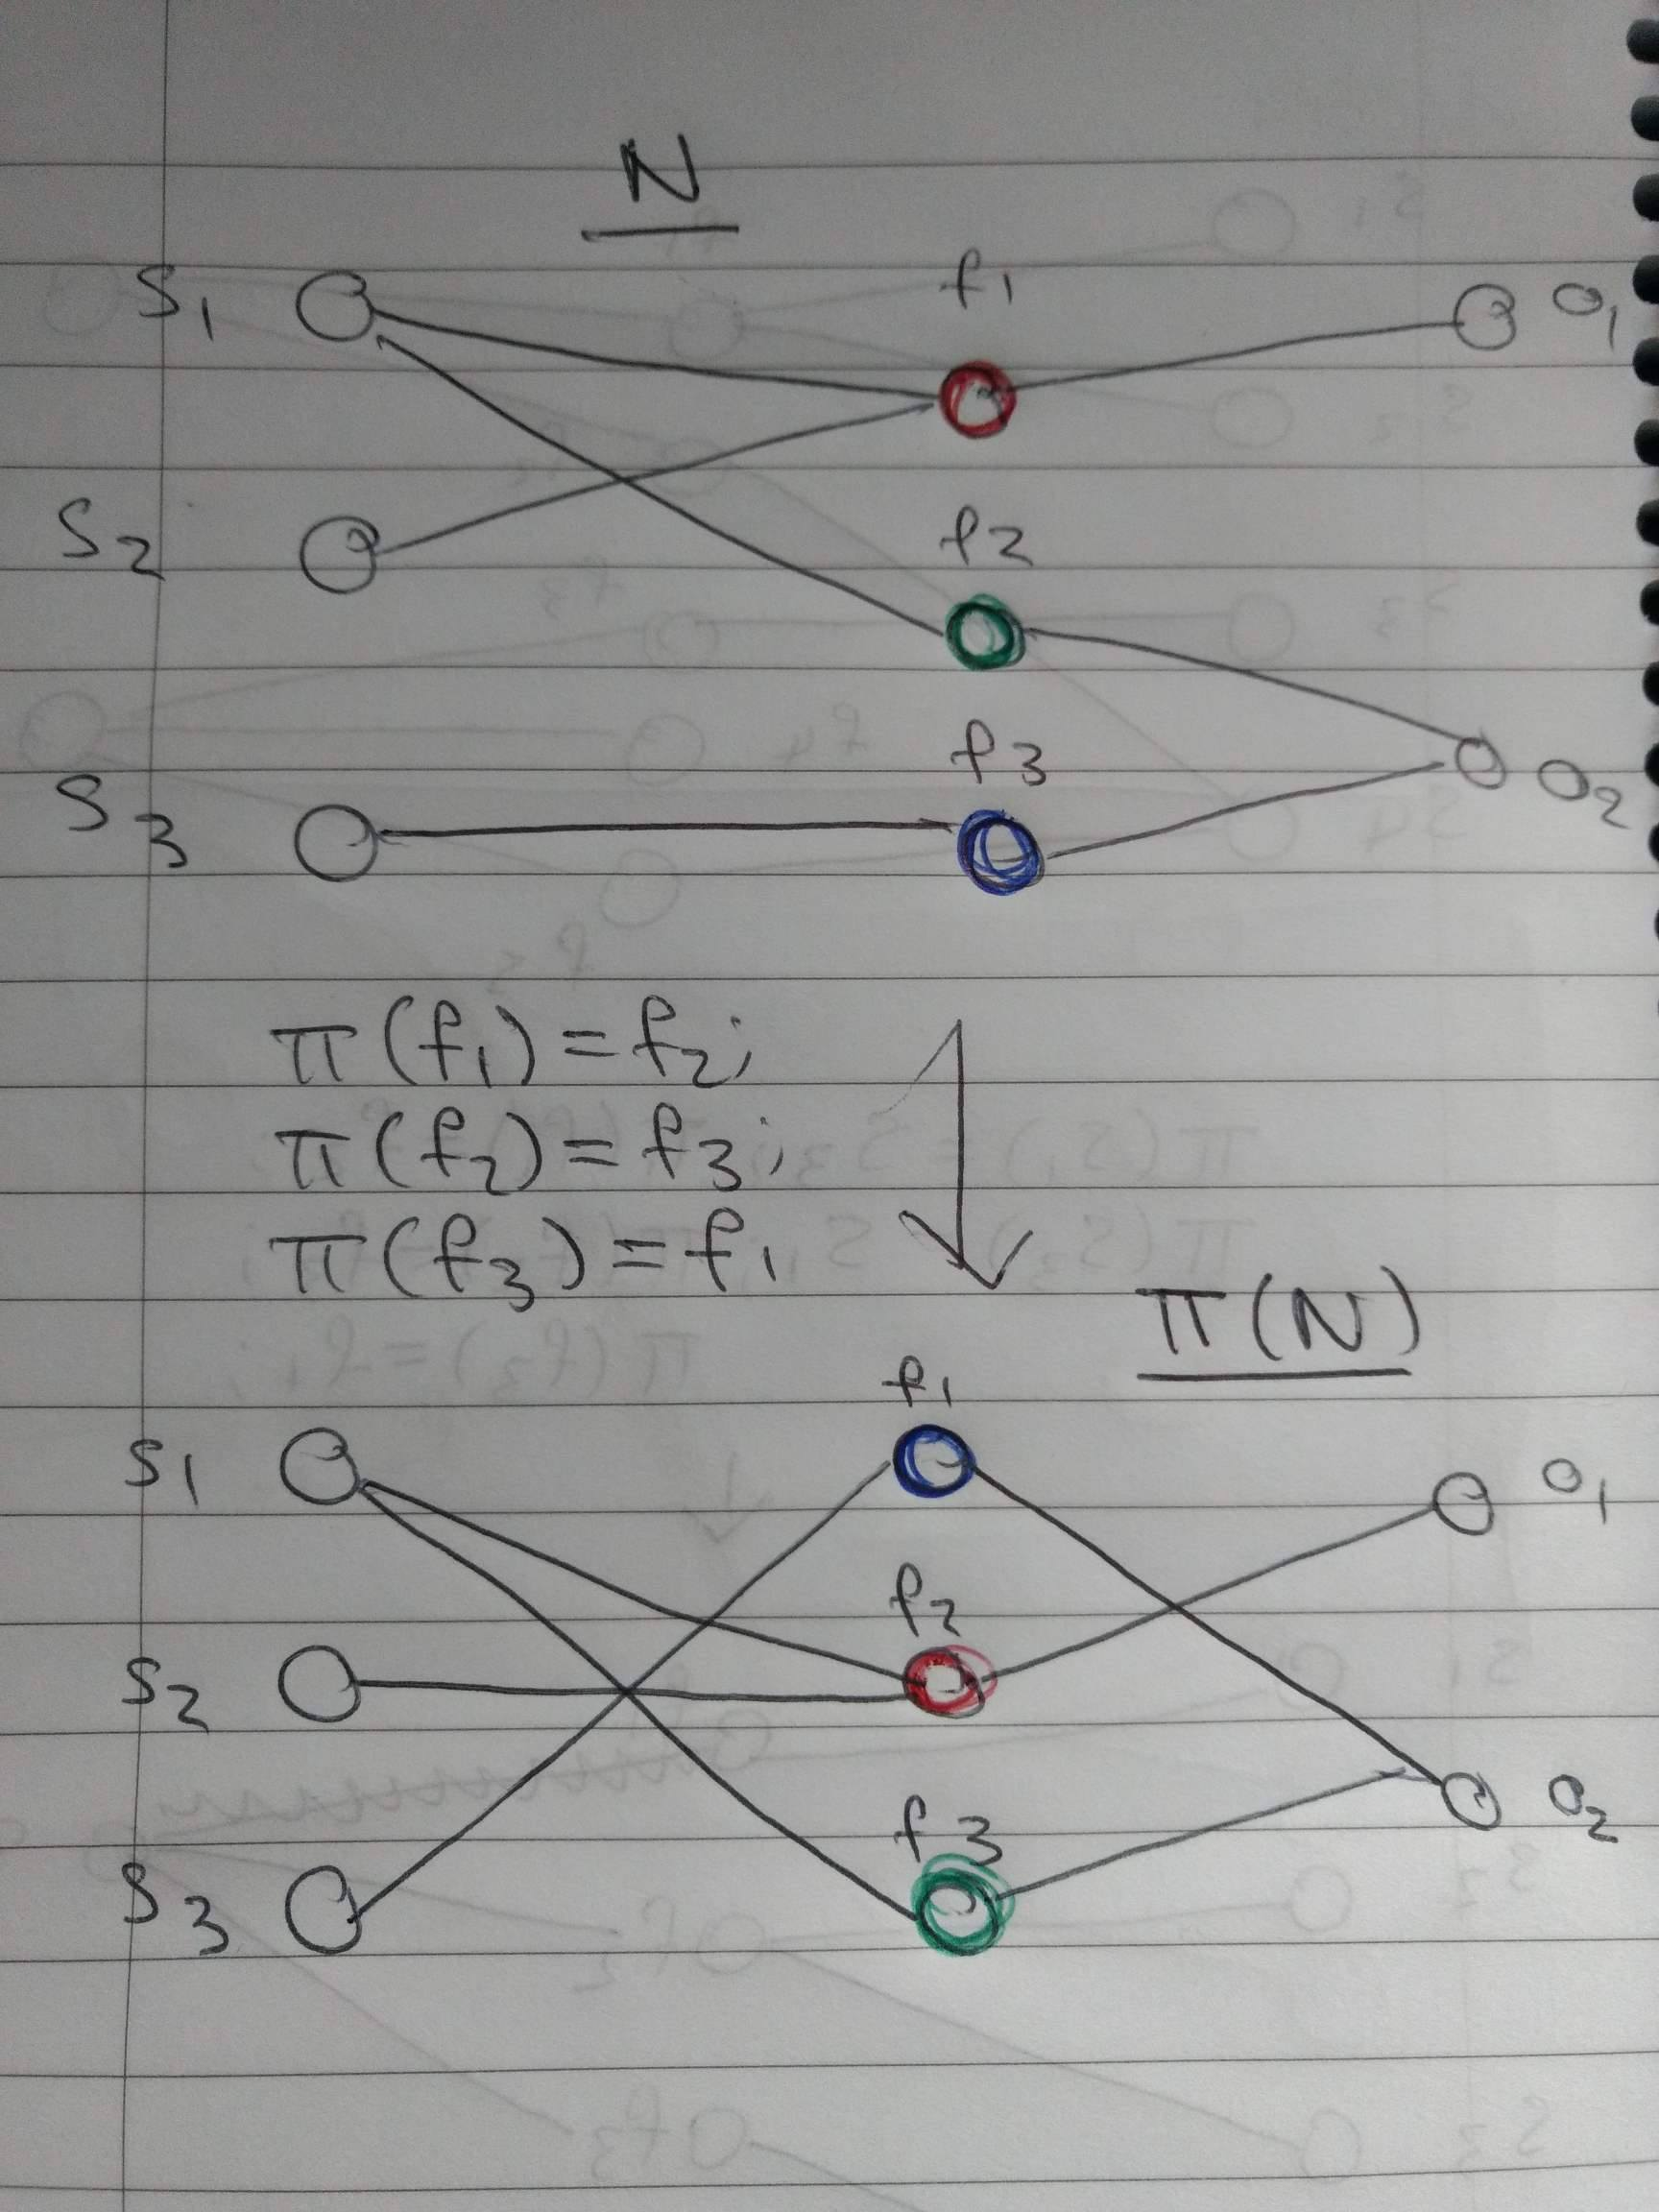
\includegraphics[width=\linewidth]{symmetry_example}
    \captionof{figure}{Example of a permutation of a truth-discovery network}
    \label{img:permutation_of_a_tdn}
}

\bibliography{references}{}
\bibliographystyle{plain}

% \end{multicols}

\appendix
\section{Proofs}

\subsection{Proof of proposition \ref{prop:symm_iff_fact_source_object_symm}}
\begin{proof}

The `only if' direction is clear. For the converse, suppose $T$ is source, fact
and object symmetric, and let $N$, $N'=\pi(N)$ be equivalent networks. Define
\begin{equation*}
\pi_\S(x) = \begin{cases}
    \pi(x) & \text{ if } x \in \S \\
    x      & \text{ if } x \in \F \cup \O
\end{cases}
\end{equation*}
Define $\pi_\F$, $\pi_\O$ similarly, and set $\sigma = \pi_\S \circ \pi_\F
\circ \pi_\O$. Then for $s \in \S$,
\begin{align*}
\sigma(s) &= \pi_\S(\pi_\F(\pi_\O(s))) \\
          &= \pi_\S(\pi_\F(s)) \\
          &= \pi_\S(s) \\
          &= \pi(s)
\end{align*}
Similarly $\sigma(f)=\pi(f)$ and $\sigma(o)=\pi(o)$ for $f \in \F$ and $o \in
\O$. Hence $\sigma=\pi$.

Let $s_1, s_2 \in \S$. Since $\pi_\O$ only permutes objects, we may apply
object-symmetry to get
$$ s_1 \sle_N^T s_2 \iff \pi_\O(s_1) \sle_{\pi_\O(N)}^T \pi_\O(s_2) $$
Then since $\pi_\F$ only permutes facts and $\pi_\S$ only permutes sources, we
may successively apply fact and object symmetry to the right hand side to get
\begin{align*}
s_1 \sle_N^T s_2 & \iff \sigma(s_1) \sle_{\sigma(N)}^T \sigma(s_2) \\
                 & \iff \pi(s_1) \sle_{\pi(N)}^T \pi(s_2) \\
                 & \iff \pi(s_1) \sle_{N'}^T \pi(s_2)
\end{align*}
An identical argument for fact ranking gives $f_1 \fle_N^T f_2 \iff \pi(f_1)
\fle_{N'}^T f_2$. Hence $T$ is symmetric.

\end{proof}

\subsection{Proof of proposition \ref{prop:same_facts_ranked_equally}}
\begin{proof}

For the first claim, consider the permutation $\pi = (s_1, s_2)$. We claim that
$\pi(N) = N$. Let $E$ be the edges in $N$ and $\pi(E)$ be the edges in
$\pi(N)$. For any $(s, f) \in \S \times \F$ we have three cases:
\begin{enumerate}
\item $s \notin \{s_1, s_2\}$: in this case $(\pi(s), \pi(f)) = (s, f)$ and
$(s, f) \in E$ iff $(\pi(s), \pi(f)) \in \pi(E)$ by definition, so
$(s, f) \in E$ iff $(s, f) \in \pi(E)$.

\item $s=s_1$: Here we have $(s_1, f) \in E$ iff $(s_2, f) \in E$ by
hypothesis. This is equivalent to $(\pi(s_2), \pi(f)) \in \pi(E)$ by definition
of $\pi(E)$, which by definition of $\pi$ is equivalent to $(s_1, f) \in
\pi(E)$.

\item $s=s_2$: As above, $(s_2, f) \in E$ iff $(s_2, f) \in \pi(E)$
\end{enumerate}
Also, it is clear that $(f, o) \in E$ iff $(f, o) \in \pi(E)$ for $f \in \F$,
$o \in \O$. We have shown that $(x, y) \in E$ iff $(x, y) \in \pi(E)$, ie.
$\pi(E) = E$ and thus $\pi(N) = N$. Applying source-symmetry, this gives
\begin{align*}
    s_1 \sle_N^T s_2 & \iff \pi(s_1) \sle_{\pi(N)}^T \pi(s_2) \\
                     & \iff s_2 \sle_N^T s_1
\end{align*}
i.e. $s_1 \seq_N^T s_2$.

For the second claim, consider $\sigma = (f_1, f_2)$ and apply a similar
argument to the above. Note that we require $f_1$ and $f_2$ to be associated
with the same object here so that both facts have the same incoming and
outgoing edges in $N$.

\end{proof}

\subsection{Proof of proposition \ref{prop:symm_and_dict}}
\begin{proof}

Suppose $T$ is source-symmetric and a dictatorship with dictator $s^*$. Let
$N=(V,E)$ be a truth-discovery network.
\begin{enumerate}
\item
    Let $s_1, s_2 \in \S$. Without loss of generality $s_1 \sle_N^T s_2$, since
    $\sle_N^T$ is complete. Consider the permutation $\pi=(s_1, s^*)$.  We have
    $s_2 \sle_{\pi(N)}^T s^*$ by dictatorship in $\pi(N)$, which by symmetry
    means $\pi^{-1}(s_2) \sle_N^T \pi^{-1}(s^*)$, i.e. $s_2 \sle_N^T s_1$.
    Hence $s_1 \seq_N^T s_2$ as required.

\item
    Let $f_1, f_2 \in \F$ such that there is a source $s$ with $(s, f_1) \in E$.
    Set $\sigma=(s, s^*)$. Then $\sigma(E)$ contains $(\sigma(s), \sigma(f_1))
    = (s^*, f_1)$, so we have $\sigma(f_2) \fle_{\sigma(N)}^T f_1 =
    \sigma(f_1)$ since the facts claimed by $s^*$ rank above all others.
    Applying symmetry gives $f_2 \fle_N^T f_1$ as required.
\end{enumerate}

This implies there is no source-symmetric strict dictatorship. If $T$ were such
an operator then $T$ is also a non-strict dictatorship, so symmetry implies
all sources are ranked equally, but this contradicts $s \slt_N^T s^*$ for all
$s \ne s^*$.

\end{proof}

\subsection{Proof of proposition \ref{prop:unam_ground_indep}}
\begin{proof}

An operator that saitisfies unanimity but not groundedness is $T$ that ranks
facts according to the function
$$
    r_N(f) = \begin{cases}
        1 & \text{ if } \src(N, f) \in \{\S, \emptyset\} \\
        0 & \text{ otherwise}
    \end{cases}
    \quad (f \in \F)
$$
i.e. $f_1 \fle_N^T f_2$ iff $r_N(f_1) \le r_N(f_2)$ (note that $T$'s ranking of
sources is irrelevant). Clearly $T$ saitsfies unanimity but not groundedness:
consider any network $N$ in which there is a fact $f_1$ with no corresponding
sources, and a fact $f_2$ with at least one source, but whose sources are not
the whole of $\S$. Then $f_1 \not\fle_N^T f_2$ contrary to the requirements of
groundedness.

Reversing the fact ordering of $T$ gives an operator satisfying groundedness
but not unanimity.

\end{proof}

\end{document}
